\documentclass[12pt,a4paper,twoside]{article}
\usepackage{labor}
\begin{document}

%fill for cover and header creation
\newcommand\laboratorynumber{2}
\title{Spektralphotometer}
\newcommand\supervisor{Ditlbacher, Harald}
\newcommand\groupnumber{42}

\newcommand\participantonelastname{Eisner}
\newcommand\participantonefirstname{Nico}
\newcommand\participantoneid{12214121}
\newcommand\participanttwolastname{Waldl}
\newcommand\participanttwofirstname{Philip}
\newcommand\participanttwoid{12214120}
\author{\participantonelastname \ \& \participanttwolastname}

\newcommand\degreeid{UB 033 678}
\newcommand\semester{23WS}
\date{24.11.2023}

%select correct course title
%\newcommand\coursetitle{Einführung in die \\ physikalischen Messmethoden}
%\newcommand\coursetitle{Laborübungen 1: \\ Mechanik und Wärme}
\newcommand\coursetitle{Laborübungen 2: \\ Elektrizität, Magnetismus, Optik}
%\newcommand\coursetitle{Fortgeschrittenen Praktikum 1: \\ Technische Physik}
%\newcommand\coursetitle{Fortgeschrittenen Praktikum 2: \\ Allgemeine Physik}

%\begin{titlepage}
   \begin{center}
       \begin{figure}[H]
            \begin{minipage}[h]{30mm}
                \centerline{
\includegraphics[height=15mm]{cover_nudes/tugraz.png}}
            \end{minipage}
            \hfill
            \begin{minipage}[h]{30mm}
                \centerline{
\includegraphics[height=15mm]{cover_nudes/nawi_graz.png}}
            \end{minipage}
            \hfill
            \begin{minipage}[h]{30mm}
                \centerline{
\includegraphics[height=15mm]{cover_nudes/uni-graz.png}}
            \end{minipage}
        \end{figure}
        
        \large{\emph{Institut für Experimentalphysik der Technischen Universität Graz \\
        \& Institut für Physik der Universität Graz}} \\
        \vspace{5mm}
        
        {\Huge \textbf{\coursetitle}}
        \vspace{5mm}
        
        {\huge \laboratorynumber: \thetitle}
    \end{center}
    
    \vfill
    
    \begin{table}[H]
        \LARGE
        \centering
        \begin{tabular}{r l}
            Betreuer:       & \supervisor \\
            Gruppennummer:  & \groupnumber \\
            \\
            Name:           & \participantonelastname, \participantonefirstname \\
            Matrikelnummer: & \participantoneid \\
            Name:           & \participanttwolastname, \participanttwofirstname \\
            Matrikelnummer: & \participanttwoid \\
            \\
            Kennzahl:       & \degreeid \\
            Datum:          & \semester \ | \thedate
        \end{tabular}
    \end{table}
    \vspace{4cm}
\end{titlepage}
\clearpage
\setcounter{page}{1}

%\maketitle %short title alternative

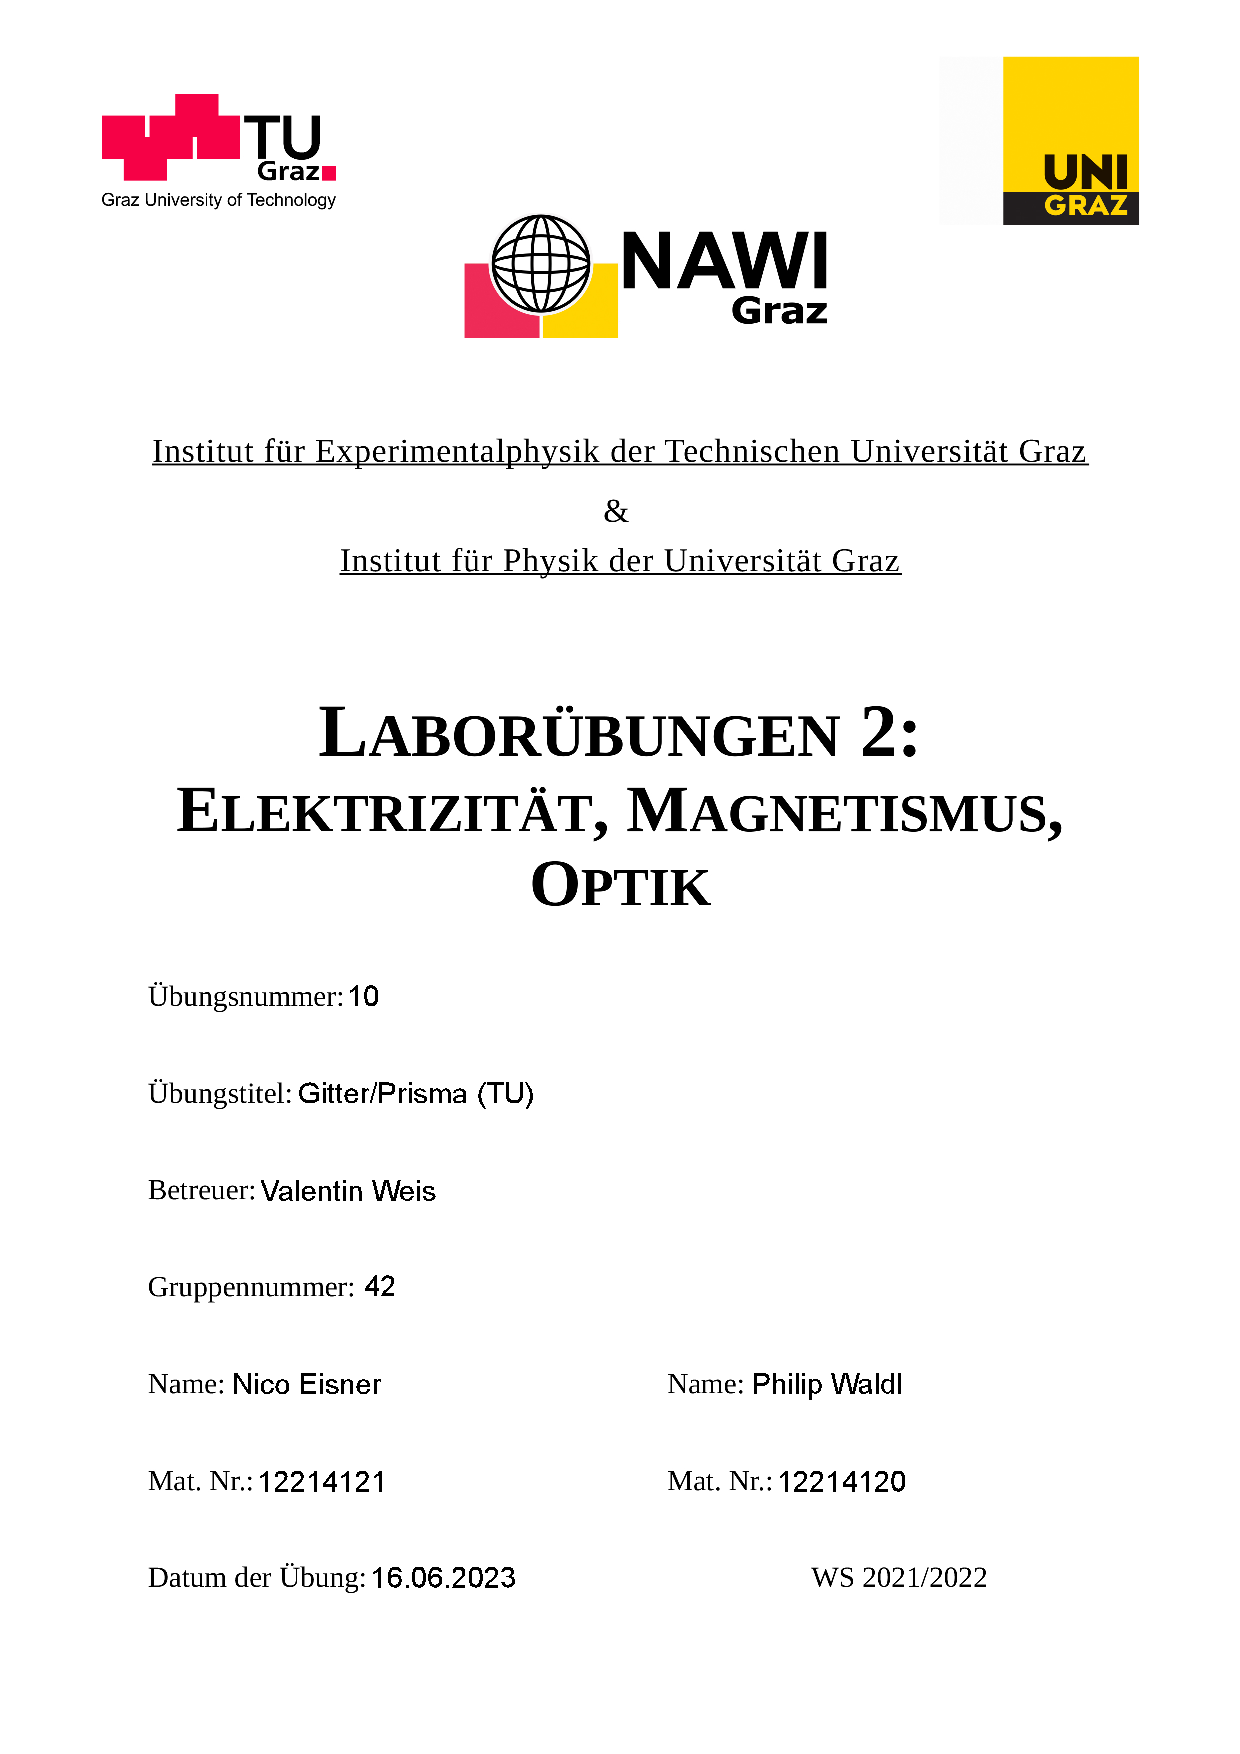
\includepdf[pages={1}]{../Deckblätter/Deckblatt_Gitter.pdf}

\tableofcontents
\newpage

\section{Aufgabenstellung} %jo beschreibn wos gmocht host ------------------------------
Der Versuch Spektralphotometer beschäftigt sich, wie der Name bereits vermuten lässt, mit dem Spektralphotometer. Dabei wird vor allem Wert auf das feststellen von Transmission- und optischer Extinktion gesetzt. 
Mit diesen Tools können weiters einige andere Größen bestimmt werden, wie beispielsweiße die Stoffemengenkonzentration und Dicke von verschiedenen Proben. \newline

\noindent
Die genaue Aufgabenstellung sieht wie folgt aus: 

\begin{itemize}
    \item Messen der optischen Transmissionen von Farbfiltern mittels Spektralphotometer
    \item Zeigen der Additivität der Extinktion anhan zweier Farbfiltern
    \item Bestimmung der Stoffemengenkonzentration von Methylenblaulösung
    \item Diskussion des Farbeindrücke der jeweilig gemessnen Spektren
    \item Messung der Glasplattendicke durch Auswertung der Transmissionsmaxima
\end{itemize}

\noindent
Alle Informationen und Methodiken wurden uns von der Technischen Universität bereitgestellt \cite{teachcenter2}. 



\section{Voraussetzungen \& Grundlagen} %Grundlagen erklären, Formeln mit erklärung

Wie im Kapitel Aufgabenstellung bereits erwähnt, dreht sich bei diesem Versuch beinahe alles um das Spektralphotometer. Dieses wissenschaftliche Messinstrument wird verwendet, um die Lichtintensitäten von verschiedenen Bereichen des elektromagnetischen Spektrums zu messen. Dabei finden sich Anwendungsmöglichkeiten in fast jeden naturwissenschaftlichen Bereichen.
Der grundlegende Aufbau eines solchen optischen Instrumentes ist in folgender Abbildung \ref{fig:SpektralphotometerAufbau} ersichtlich.

\begin{figure}[H]
    \centering
    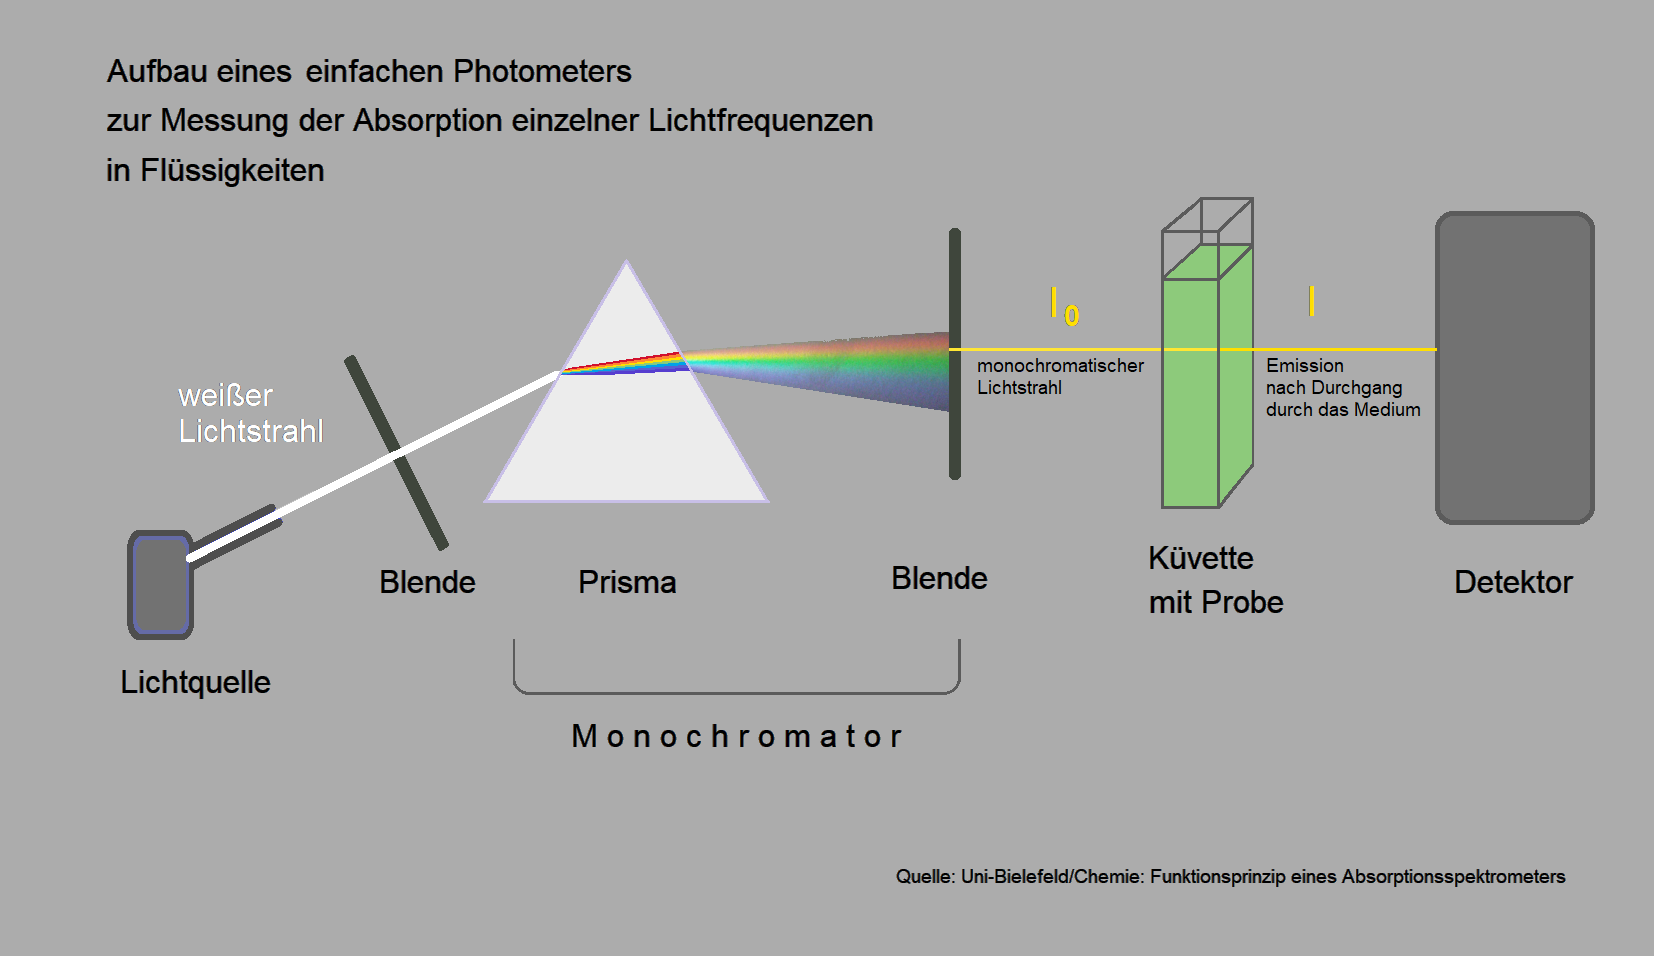
\includegraphics[width=0.6\linewidth]{nudes/SpektralphotometerAufbauWiki.png}
    \caption{Grundlegender Aufbau eines Spektralphotometer \cite{SpektralphotometerWiki}}
    \label{fig:SpektralphotometerAufbau}
\end{figure}

\noindent
Wie sich erkennen lässt, bildet ein Monochromator, genauer der Czerny-Turner-Monochromator, das Herzstück des Spektralphotometers. Dieser sorgt dafür, dass das eingehende Licht der Lichtquelle in ihre einzelnen Farbspektren zerlegt werden. Mit einer Blende wird dann nur eine der Farbstrahlen an die Probe und in weiterer Folge an den Detektor durchgelassen. 
Die Intensität des Lichtstrahles, welcher vom Monochromator auf die Probe trifft, ist die einfallende Lichtintensität $I_{0}$, die Intensität des Strahls nach der Probe $I_{T}$ ist jene vom transmittierten Lichtes durch die Probe.
Der eben genannte Monochromator sieht in vereinfachter Darstellung so aus:

\begin{figure}[H]
    \centering
    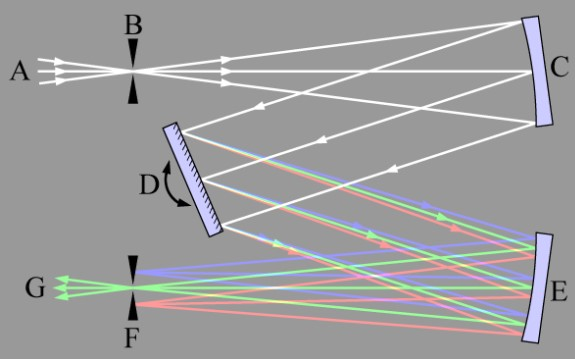
\includegraphics[width=0.6\linewidth]{nudes/MonochromatorAufbau.jpg}
    \caption{Grundlegender Aufbau eines Czerny-Turner-Monochromators}
    \label{fig:MonochromatorAufbau}
\end{figure}

\noindent
Das Licht trifft hierbei von der Quelle A durch eine Blende B auf einen Hohlspiegel C, welcher die Strahlen auf ein schwenkbares optisches Prisma/Gitter D leitet, wo sie in ihre einzelnen Spektren aufgeteilt wird.
Von dort wird das Licht auf einen weiteren Hohlspiegel E gelenkt. Dadurch, dass die abgespalteten Farbstrahlen durch das Prisma/Gitter je nach Neigung unterschiedlich abgelenkt werden, kann durch justieren der Prisma-/Gitterneigung jenes Farbspektrum bestimmt werden, welches den Monochromator durch ein Blende F verlassen und zum Detektor G weitergeleitet werden darf. \newline

\noindent
Da die grundlegende Funktionsweiße des Spektralphotometers nun bekannt ist, wird es Zeit, sich mit einigen Begriffen im Zusammenhang mit dem Messgerät und dessen Einsatz bekannt zu machen:


\subsection{Transmission,Extinktion und Absorptionsquerschnitt}

Farben sind im Grund nichts anderes, als die unterschiedliche Reflexion, Absorption und Streuung von verschiedenen Wellenlängen des Lichtes aufgrund der chemischen und physikalischen Eigenschaften des Materials. 
Scheint Licht also auf einen teiltransperenter Körper, so wird ein Teil davon durch diesen hindurchgehen, was als Transmission T bezeichnet wird. Diese setzt sich aus dem Verhältnis der Lichtintensität des eingehenden Strahles $I_{0}$ zur Intensität des transmittierten Strahlen $I_{T}$ zusammen, als Gleichung formuliert in Formel \ref{eq:Transmission}.

\begin{equation}
    \label{eq:Transmission}
    \centerline{$T=\frac{I_{T}}{I_{0}}$}
\end{equation}

\noindent
In der Spektroskopie wird jedoch meist mit logarithmischen Werten als Maß für die Lichtabschwächung gearbeitet - der Extinktion E.

\begin{equation}
    \label{eq:Extinktion}
    \centerline{$E=-log(T)=-log(\frac{I_{T}}{I_{0}})=log(\frac{I_{0}}{I_{T}})$}
\end{equation}

\noindent
Bei einer Überlagerung von mehreren Extinktionen ist die resultierende Extinktion einfach die Summe der Einzelextinktionen, was auch als Additivität der Extinktionsspektren bezeichnet wird. \newline

\noindent
Der Anteil eines einzelnen Moleküls zur Extinktion wird auch als Absorptionsquerschnitt q bezeichnet, welcher sich durch folgende Gleichung beschreiben lässt:

\begin{equation}
    \label{eq:Absorptionsquerschnitt}
    \centerline{$q=\frac{\varepsilon *ln(10)}{N_{A}}$ \\ mit $N_{A}=6,02 × 10^{23} \frac{1}{mol}$}
\end{equation}

\noindent
Dieser ist jedoch nicht zwingend gleich dem Molekülquerschnittes, sondern lediglich ein Wirkungsquerschnitt.

\subsection{Referenzspektrum}

Um die optische Transmission nun bestimmen zu können ist es notwendig, zuvor das Referenzspektrum festzulegen. Dieses ist das Spektrum, welches vom Spektrograph selbst kommt und dessen Intensität somit der Größe $I_{0}$ entspricht.
Das Referenzspektrum ist also das ohne Probe gemessene Lichtspektrum des Spektralphotometers. 

\subsection{Wichtige Zusammenhänge}

Für eine erfolgreiche Auswertung des Experimentes ist sind außerdem folgende Zusammenhänge vonnöten:

\begin{equation}
    \label{eq:Wellenzahl}
    \centerline{Wellenzahl \\ $v=\frac{1}{\lambda}=\frac{m}{2n_{p}d}$ \\ $\Delta v=$}
\end{equation}

    

\section{Versuchsanordnung} %mit skizze kurz beschreiben ------------------------------

Bevor die Messungen überhaupt starten konnten musste natürlich alles richtig augebaut werden. Hierfür wurde das Spektralphotometer mit Strom versorft und in weiterer Folge mit einem Computer der Universität verbunden.
Am Spektralphotometer befindet sich außedem eine Halogen-Lichtquelle, eine Probenhalterung und ein Lichtleiter, welcher das transmittierte Licht an das Spektralphotometer weitergibt.
Am PC wurde dann die Software Splicco gestartet, welches zur grafischen Darstellung der Spektren bzw. deren export als CSV-Files dient und das optische Messgerät verbunden. 

\begin{figure}[H]
    \centering
    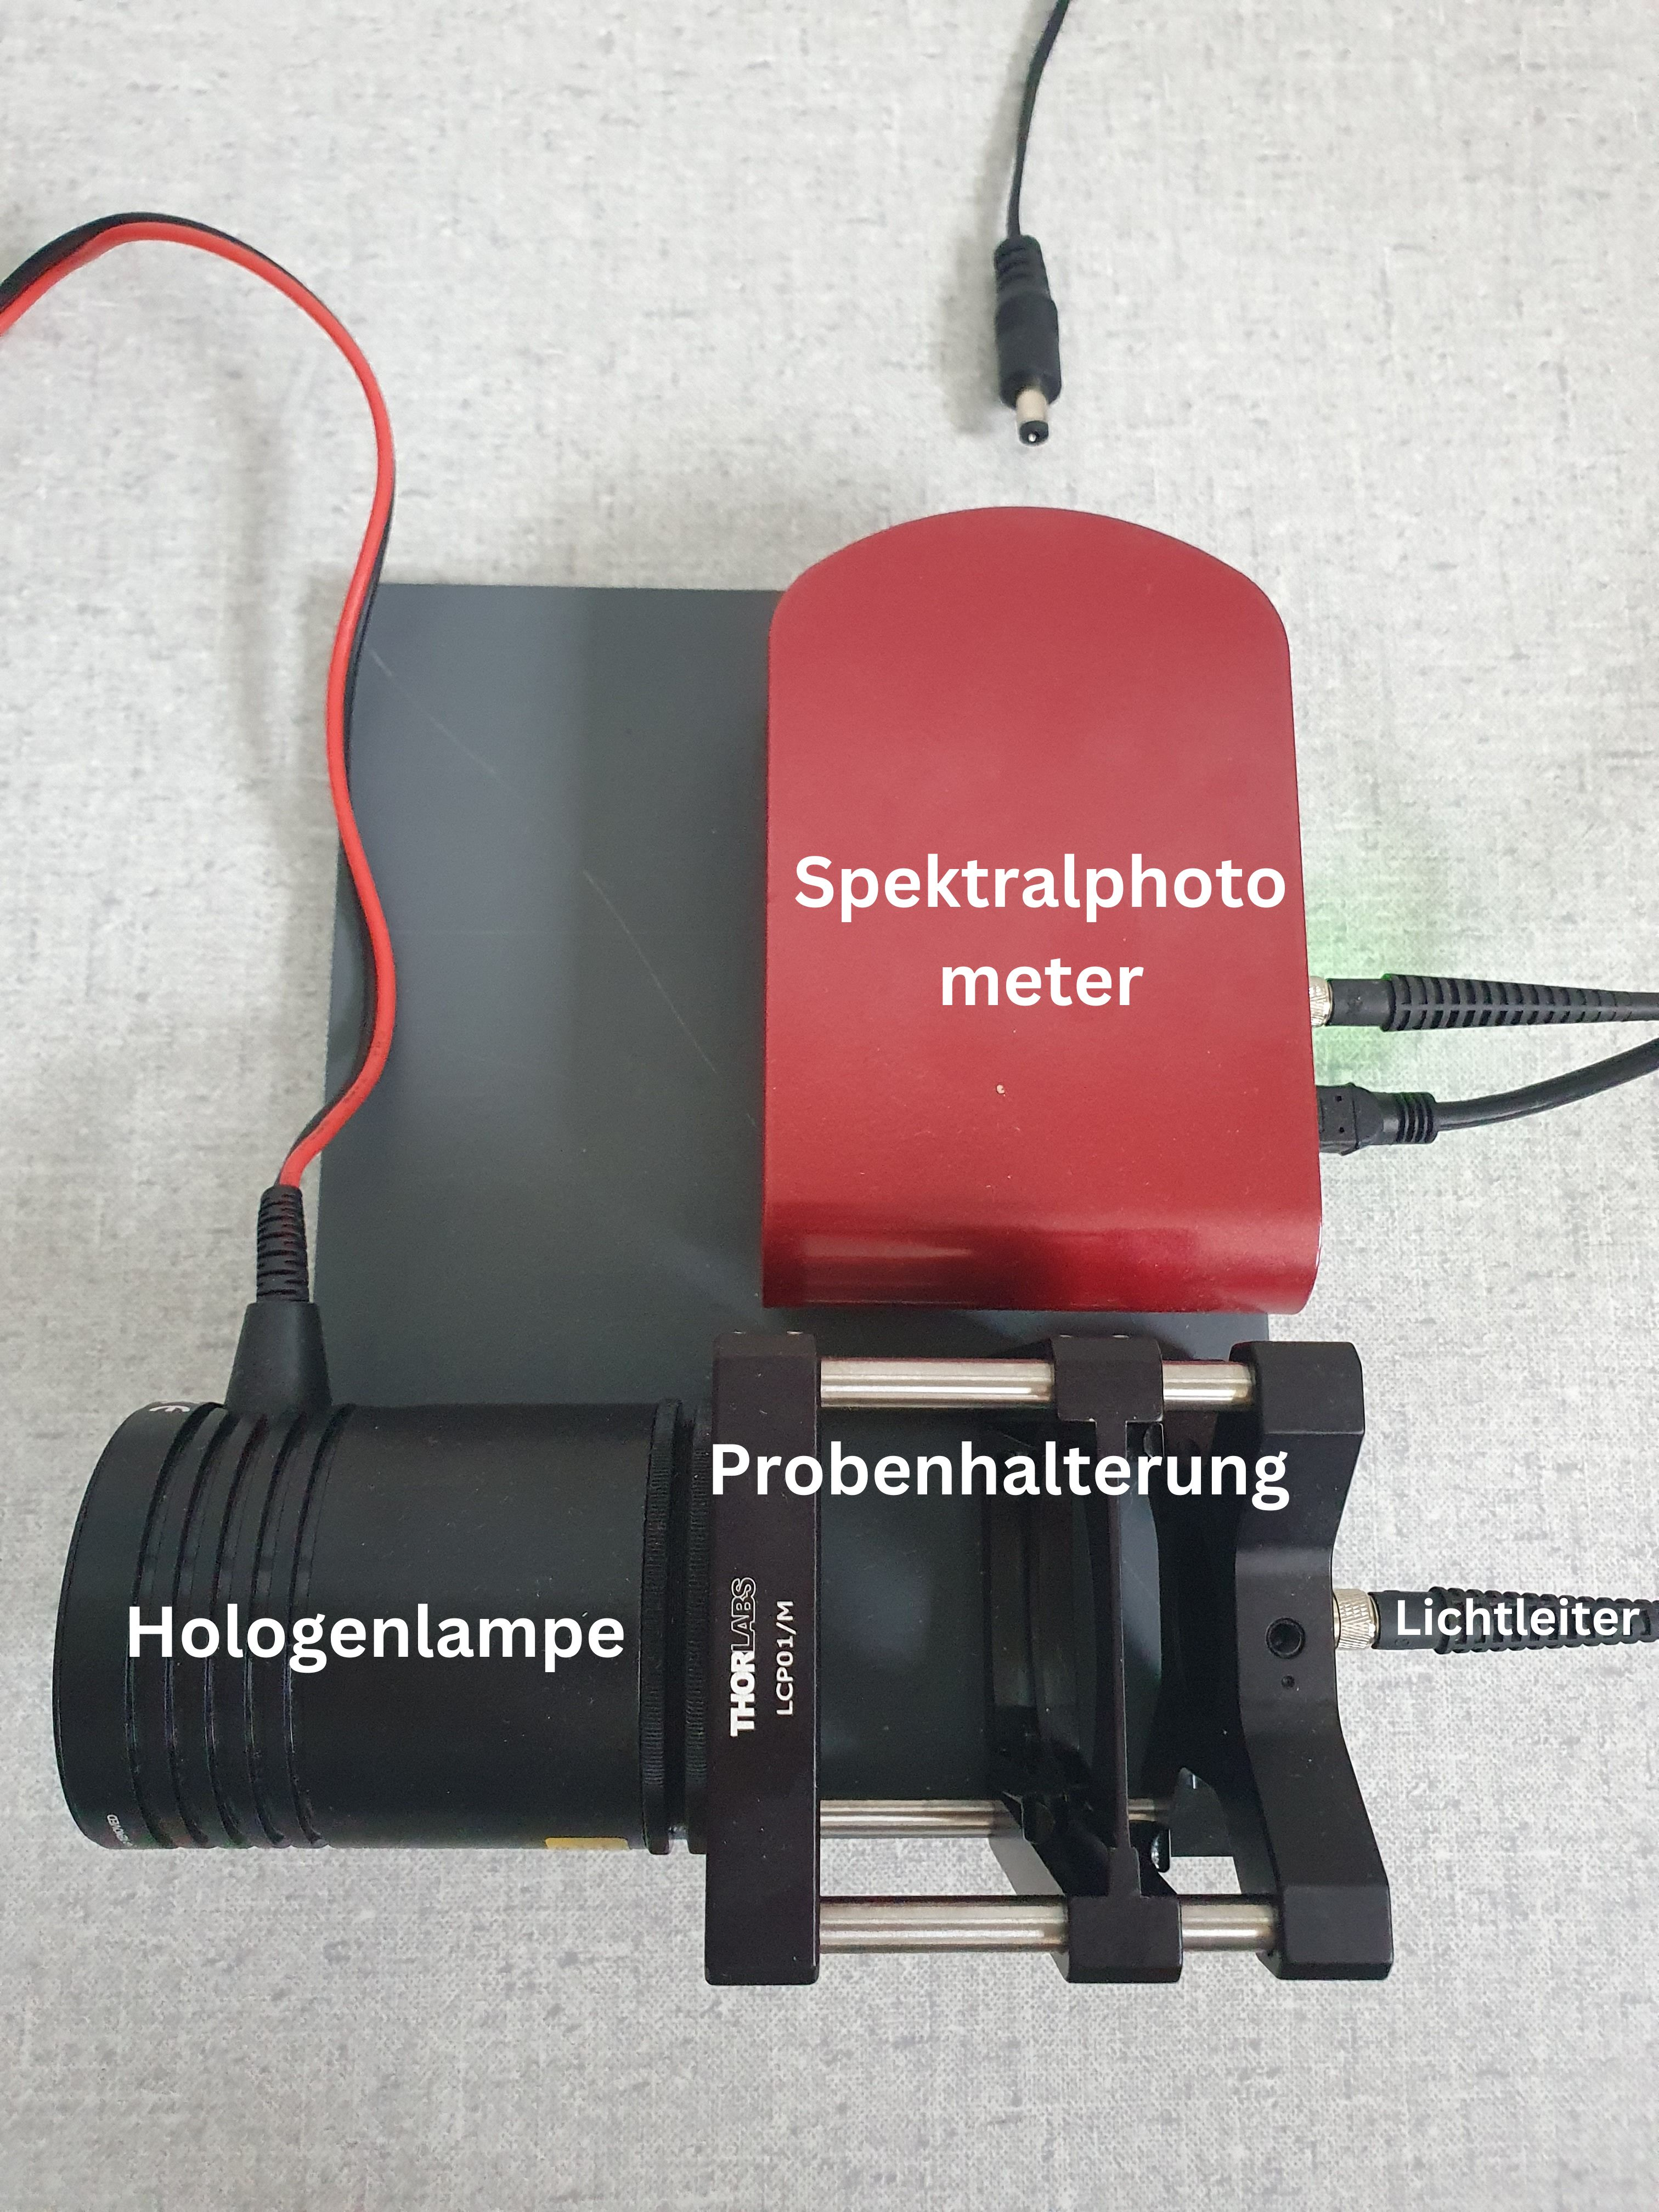
\includegraphics[width=0.6\linewidth]{nudes/Spektralphotometer.jpg}
    \caption{Aufbau Spektralphotometer}
    \label{fig:VersuchsaufbauIRL}
\end{figure}

\noindent
Nach einschalten der Hologenlampe konnten dann bereits die ersten Graphen der Lichtspektren am Monitor beobachtet werden. 

\begin{figure}[H]
    \centering
    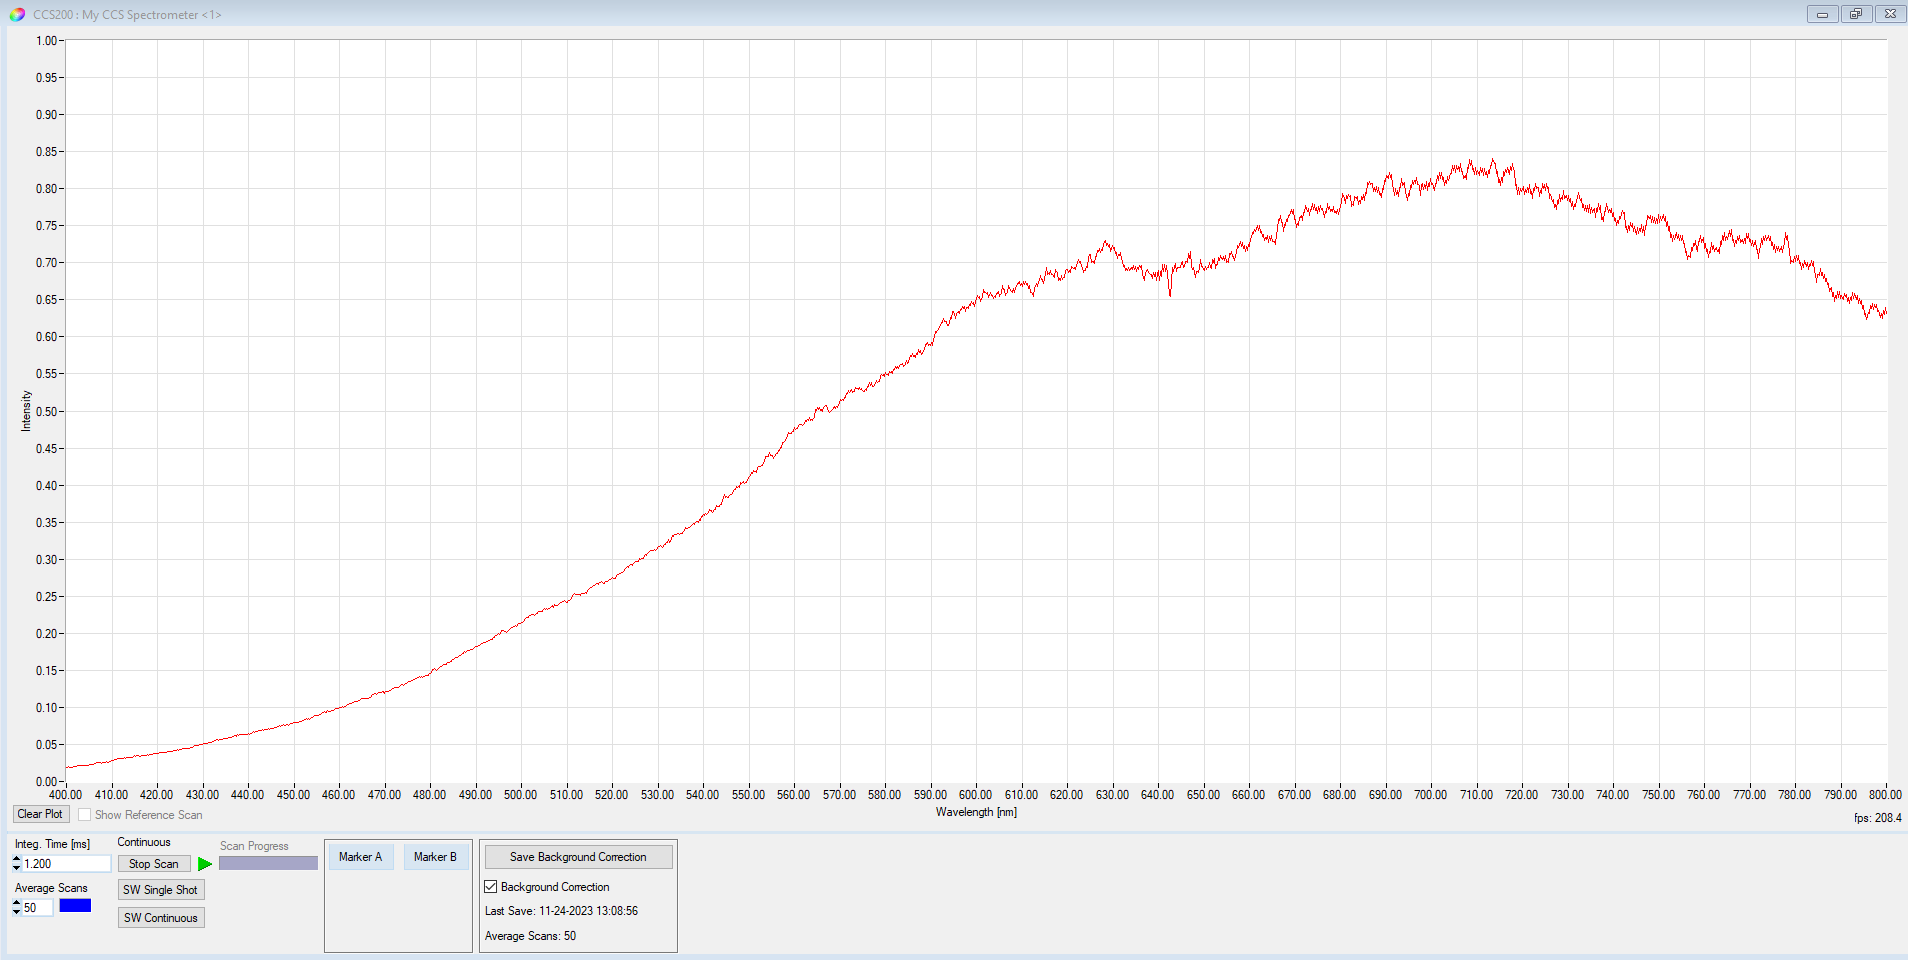
\includegraphics[width=0.6\linewidth]{nudes/Verlauf-Referenzspektrum.PNG}
    \caption{Beispiel Spektrumsdarstellung am PC}
    \label{fig:SpliccoSoftware}
\end{figure}

\noindent
Durch einsetzen von verschiedenen Proben können nun die dazugehörigen Spektren grafisch beobachtet und zur weiteren Auswertung CSV-file exportiert werden.

\begin{figure}[H]
    \centering
    \includegraphics[width=0.4\linewidth]{nudes/Proben_Farbblättchen.jpg}
    \includegraphics[width=0.3\linewidth, angle=90]{nudes/Flüssigkeitsproben.jpg}
    \caption{Proben von Farbblättchen/Glasblättchen und Wasser/Methylenblaulösung}
    \label{fig:Proben}
\end{figure}


    
\section{Geräteliste} %jo holt a listn ------------------------------

\begin{table}[H]
    \centering
    \caption{Im Versuch verwendete Geräte und Utensilien.}
    \label{tab:geraete}
    \begin{tabular}{| l | l | l |}
        \hline
        Gerät   & Gerätenummer  & Unsicherheit \\
        \hline
        Spektralphotometer & {n.a} & {n.a} \\
        Hologenlampe & {n.a} & {n.a} \\
        Probenhalterung & {n.a} & {n.a} \\
        Lichtleiter & {n.a} & {n.a} \\
        Proben & {n.a} & {n.a} \\
        PC mit Splicco-Software & {n.a} & {n.a} \\
        \hline
    \end{tabular}
\end{table}


\section{Versuchsdurchführung \& Messergebnisse} %nachvollziehbar und klar dargestellt ------------------------------

Der erste Teil des Versuches bestand daraus, die optischen Transmissionen von verschiedenen Farbfiltern mittels Spektralphotometer zu ermitteln.
Dabei wurden zunächst einige Einstellungen in der Software getätigt. Der Wellenlängenbereich wurde auf 400-800 nm beschränkt, was zienlich genau den fürs menschliche Auge sichtbaren Bereich der elektromagnetischen Strahlen (sichtbares Licht) beinhaltet.
Weiters wurde die Integrationtime auf 1.2 ms gesetzt, damit das Spektrum des Lichtes den y-Achsenbereich gut ausfüllt, aber nicht abgeschnitten wird.
Außerdem wurde der average-scans Wert noch auf 50 gesetzt. \newline

\noindent
Sobald die Software brauchbar eingestellt war, wurde eine Hintergrund-Korrektur durchgeführt. Hierfür musste lediglich die Lichtquelle abgeblendet werden, sodass jegliche Störquellen wie das Umgebungslicht, Thermische Effekte, ... die vom Spektralphotometer aufgezeichnet werden übrig bleiben. Durch einen Klick auf Save Background Correction wurde dieses Scenario dann gespeichert und von der Software bei folgenden Messungen automatisch abgezogen.
Wichtig zu beachten ist, dass die Hintergrund-Korrektur nach jedem Programmneustart oder bei einer Änderung des Umgebungslichtes bzw. der Integrationszeit zu wiederholen ist. \newline

\noindent
Folgend darauf konnten nun auch schon die ersten Messungen beginnen. Zunächst wurde das Referenzspektrum für die Intensitäten ($I_{0}$) aufgenommen. Dazu wurde einfach eine Aufnahme ohne Probe, also nur mit Halogenlampe aufgezeichnet und als CSV-Datei exportiert.
Für den Export von CSV-Daten aus Slicco wurden folgende Einstellungen für diese, als auch für alle folgenden Exporte getätigt: Seperator: Tabulator, Decimal Point ",". \newline

\noindent
Danach wurden diese Daten auch für eingesetzte Farbfilter erhoben ($I_{T}$), indem einmal ein oranger-, einmal einmal ein blauer- und schließlich beide gemeinsam eingesetzt wurden. Zur Abschätzung der Messfehler wurde dieser Vorgang (also von Referenzspektrum bis hin zu den drei Filtermessungen) fünfmal wiederholt.
Am Ende resultierten also fünfmal vier CSV-Daten der Spektren, welche in den folgenden Abbildungen grafisch dargestellt sind:

\begin{figure}[H]
    \centering
    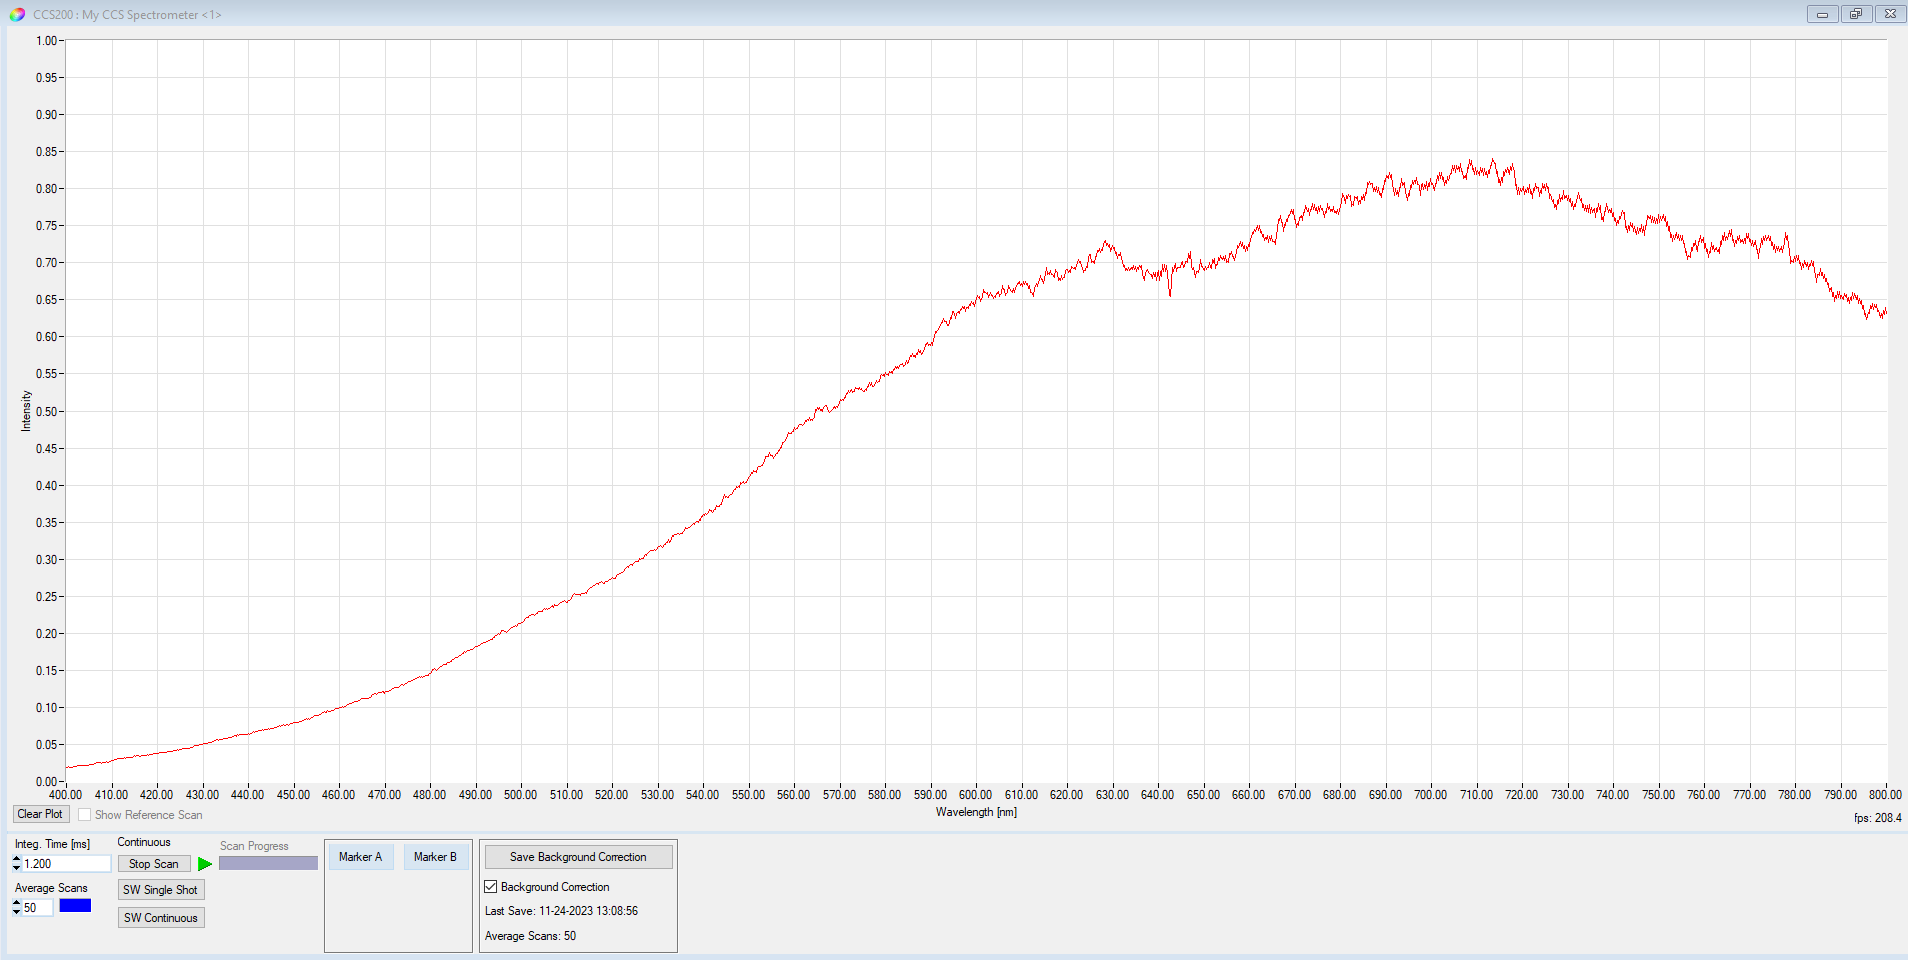
\includegraphics[width=0.4\linewidth]{nudes/Verlauf-Referenzspektrum.PNG}
    \caption{Referenzspektrum der ersten Messung}
    \label{fig:Referenzspektrum3.1Bild}
\end{figure}

\begin{figure}[H]
    \centering
    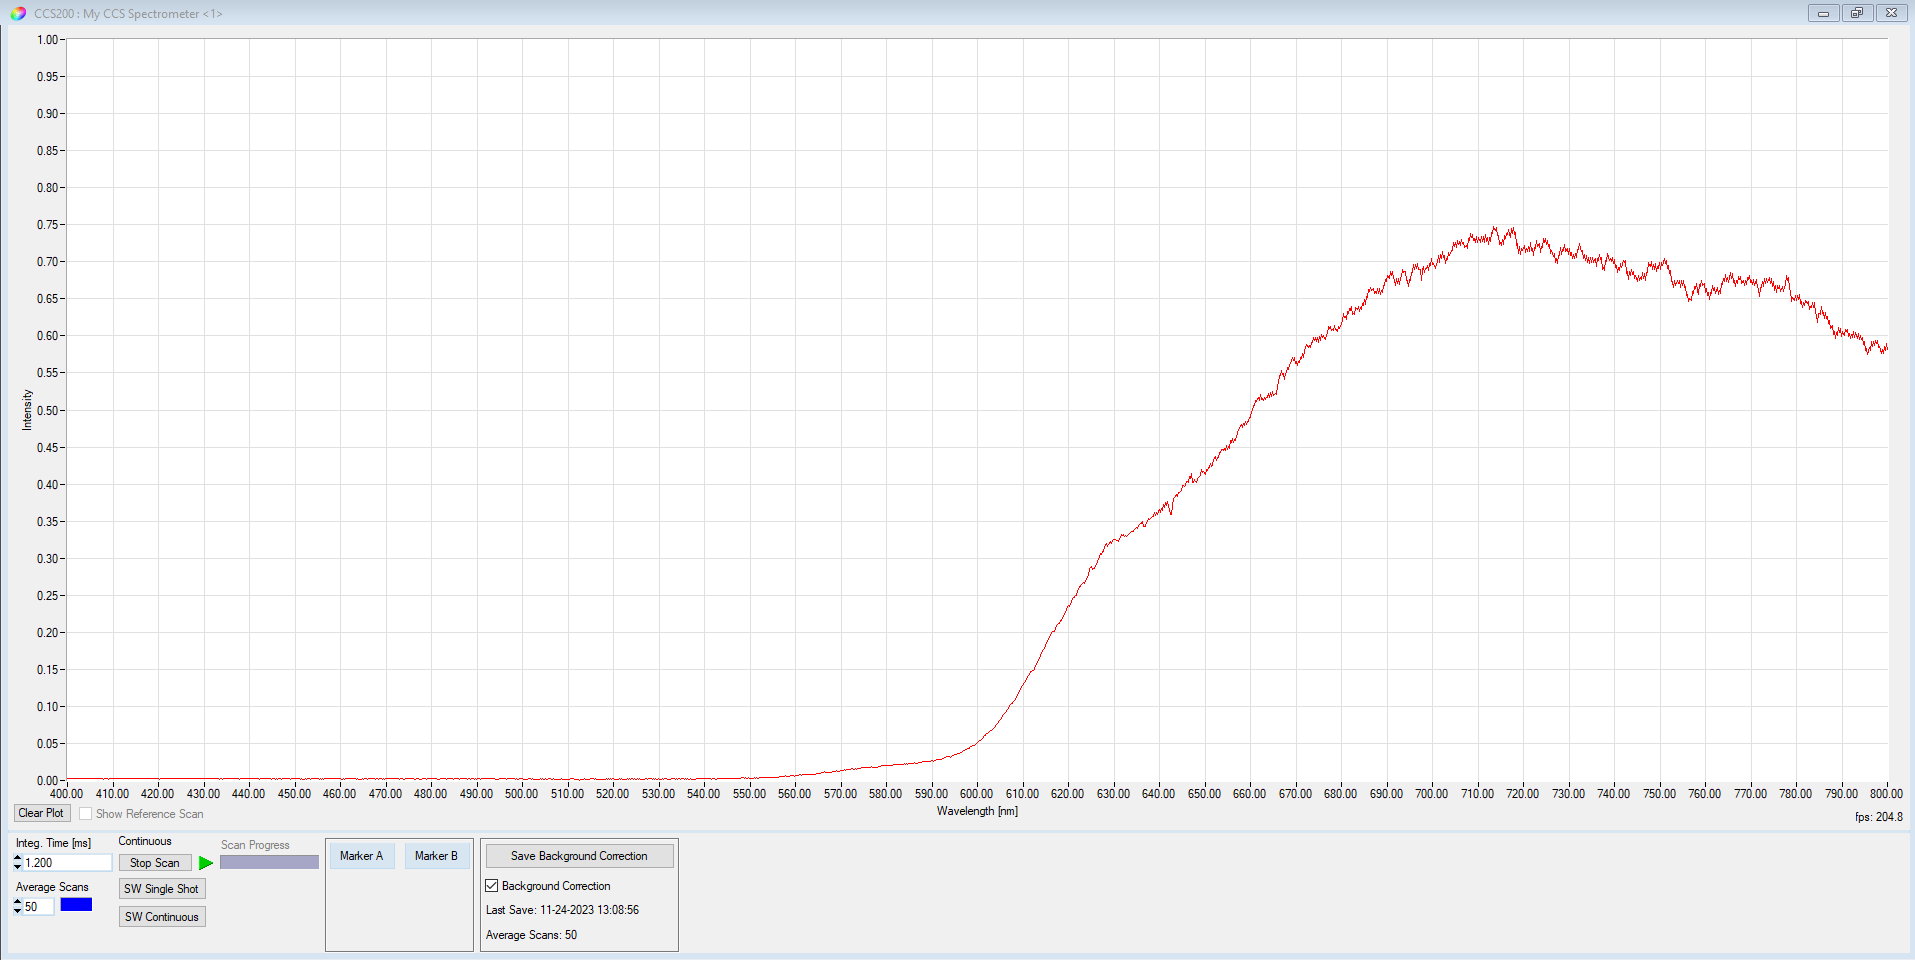
\includegraphics[width=0.4\linewidth]{nudes/Verlauf-Rot.PNG}
    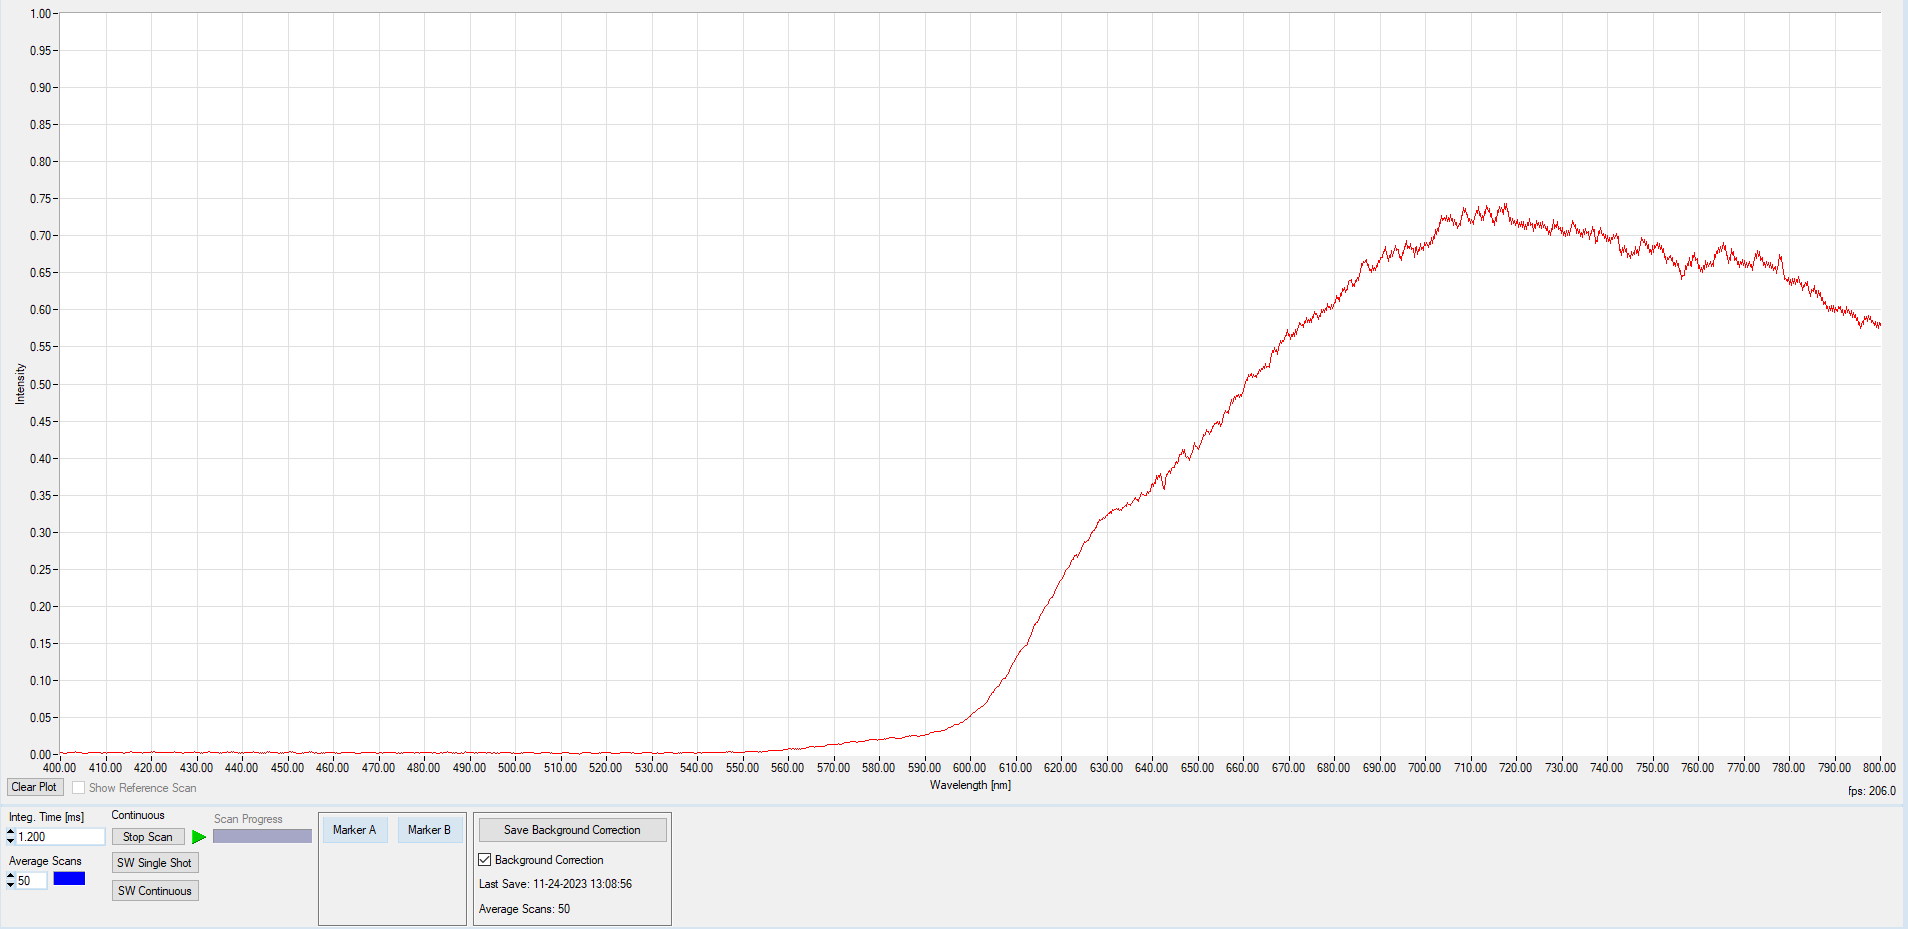
\includegraphics[width=0.4\linewidth]{nudes/Verlauf-Blau.PNG}
    \caption{Spektren des Lichtes mit oranger/blauer Filterprobe}
    \label{fig:Orange/Blau3.1Bilder}
\end{figure}

\begin{figure}[H]
    \centering
    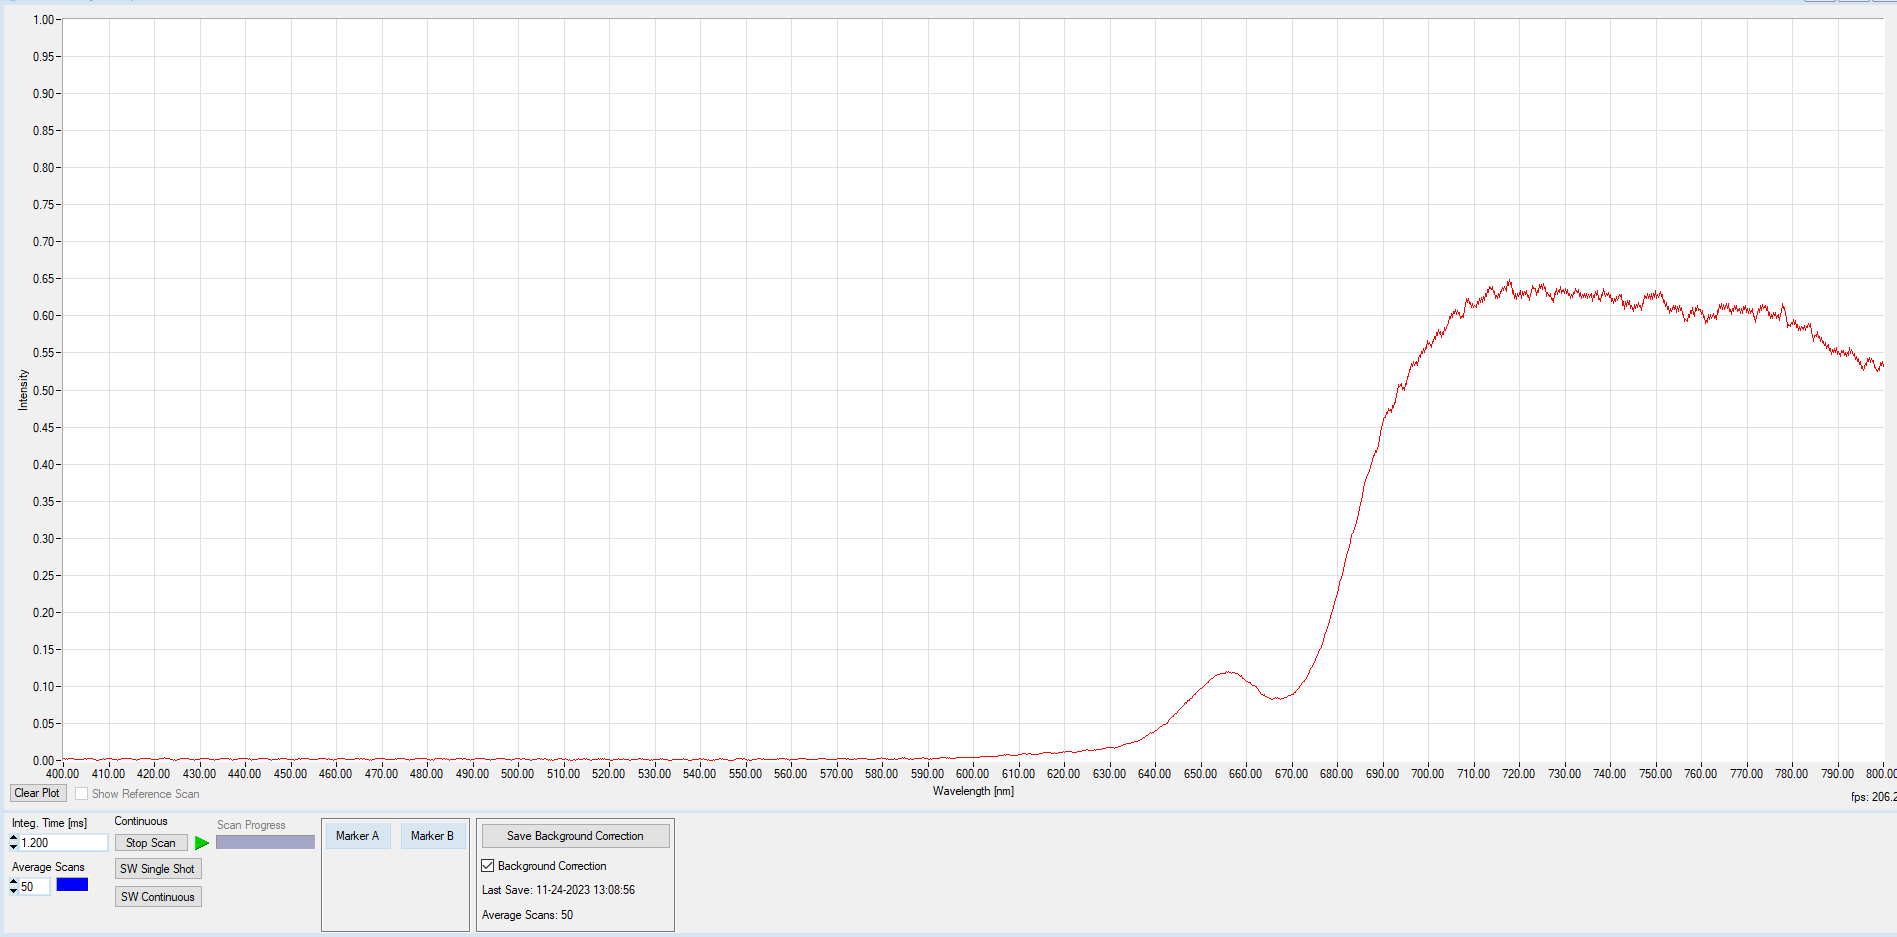
\includegraphics[width=0.4\linewidth]{nudes/Verlauf-BlauUndRot.PNG}
    \caption{Spektrum des Lichtes mit oranger und blauer Filterproben}
    \label{fig:OrangeUndBlau3.1Bilder}
\end{figure}

\begin{figure}[H]
    \centering
    \includegraphics[width=0.6\linewidth]{nudes/qti-Intensitäten-Farbfilter.jpg}
    \caption{Spektrum des Lichtes aller Messungen des Versuchsteiles mit Farbfiltern}
    \label{fig:Alle3.1Bilder}
\end{figure}


\noindent
Zur Durchführung des zweiten Versuchteiles wurden die Farbfilter dann durch Flüssigkeiten ausgetauscht. Dabei wurde zunächst Wasser als Referenzspektrum in den dafür vorgesehenen Küvettenhalter eingesetzt und als Spektrogramm dargestellt bzw. exportiert.
Danach wurde die Methylenblaulösung in die Halterung eingesetzt und die für die Auswertung wichtigen Daten gespeichert. Auch hier wurde dieser Vorgang zur Bestimmung der Unsicherheiten fünfmal wiederholt. \newline

\begin{figure}[H]
    \centering
    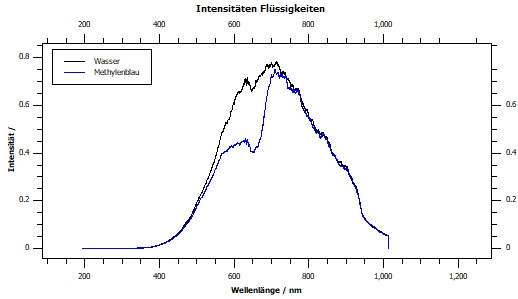
\includegraphics[width=0.6\linewidth]{nudes/qti-Intensitäten-Flüssigkeiten.jpg}
    \caption{Spektrum des Lichtes aller Messungen des Versuchsteiles mit Flüssigkeiten}
    \label{fig:Alle3.2Bilder}
\end{figure}

\noindent
Zu guter Letzt soll nun das Glasblättchen vermessen werden. Wie bereits bei den vorherigen Messungen wurde auc hier ein Referenzspektrum ohne Probe aufgenommen. Danach selbiges mit eingesetzter Probe und das ganze fünfmal wiederholt und schon waren die Messungen abgeschlossen. 

\begin{figure}[H]
    \centering
    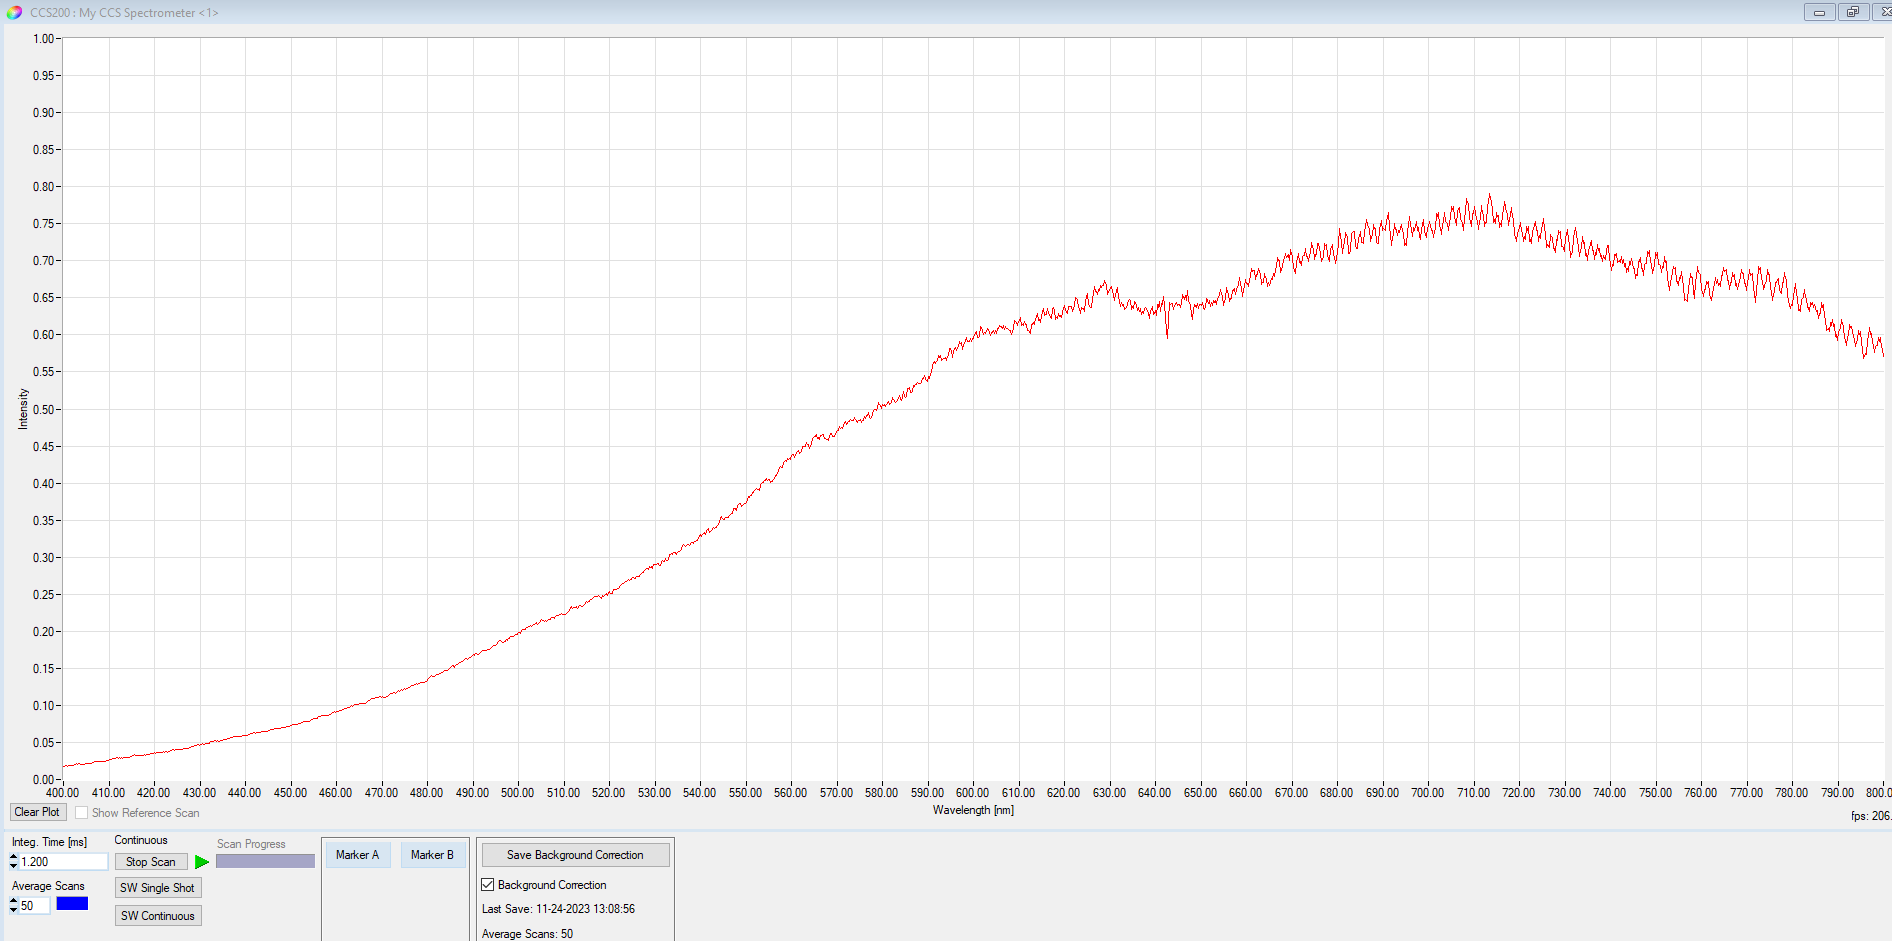
\includegraphics[width=0.4\linewidth]{nudes/Verlauf-ReferenzspektrumGlas.PNG}
    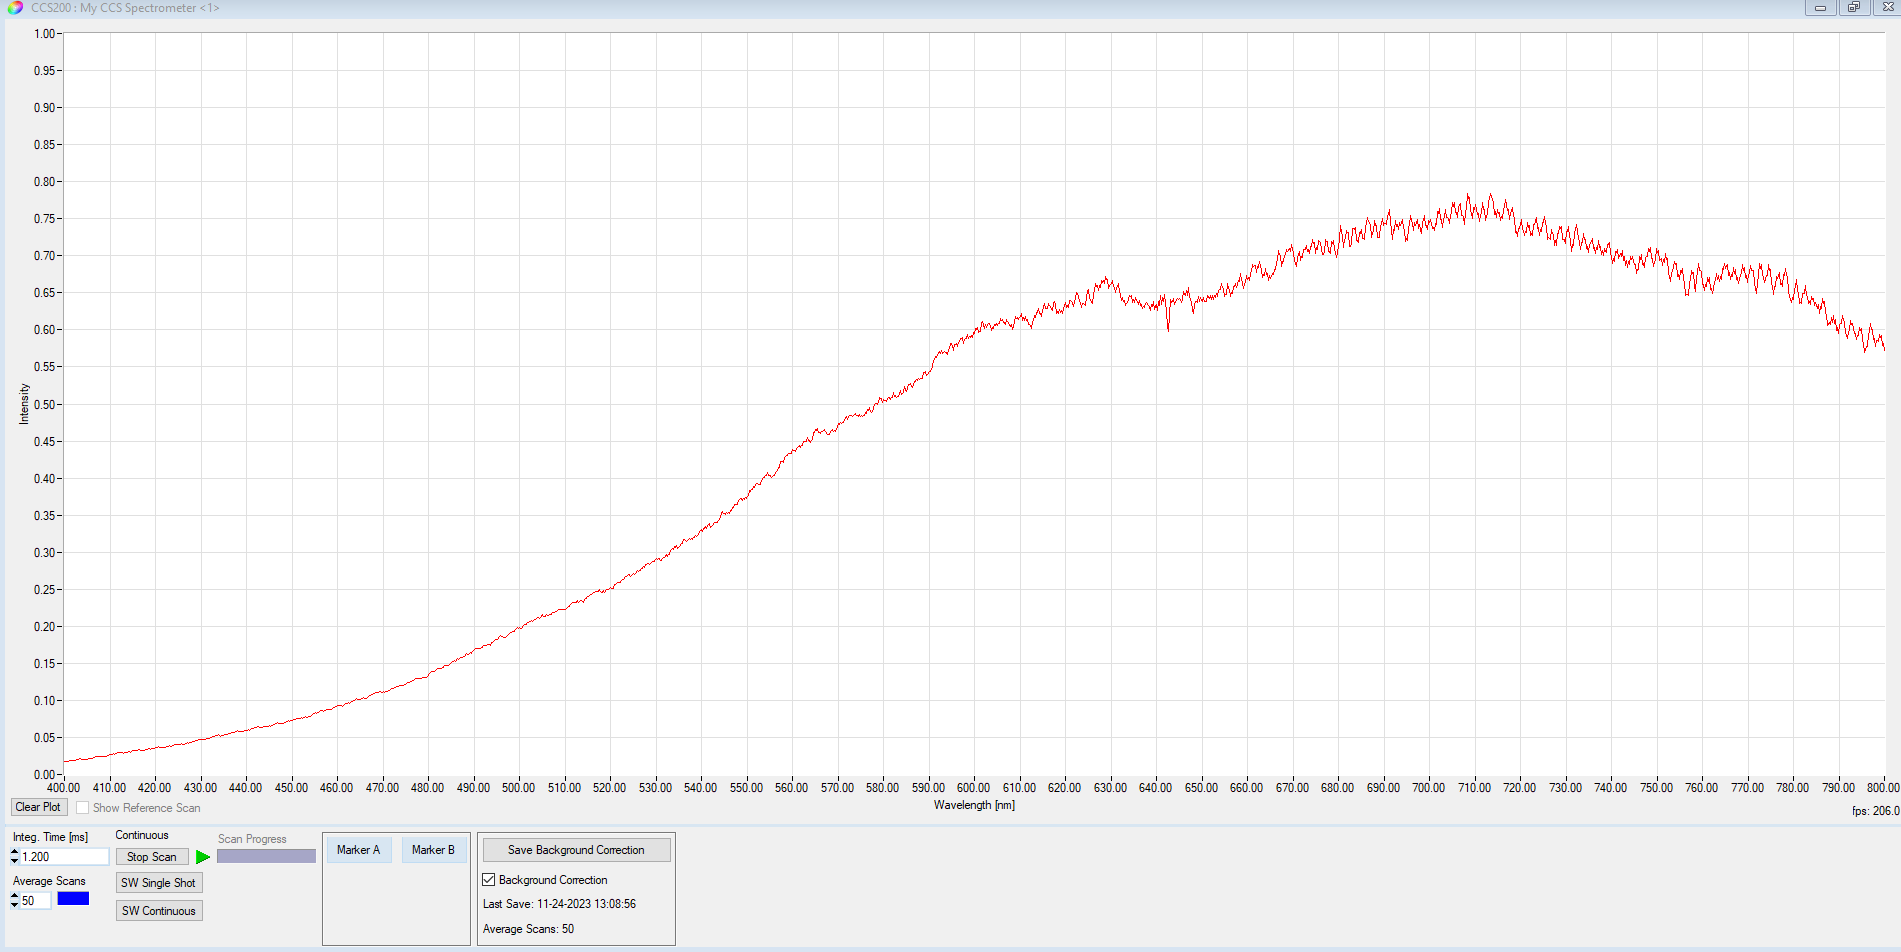
\includegraphics[width=0.4\linewidth]{nudes/Verlauf-Glas.PNG}
    \caption{Referenzspektrum für Glasblättchen / Spektrum mit eingesetztem Glasblättchen}
    \label{fig:MessungenGlas}
\end{figure}

\begin{figure}[H]
    \centering
    \includegraphics[width=0.6\linewidth]{nudes/qti-Intensitäten-Glas.jpg}
    \caption{Referenzspektrum für Glasblättchen und Spektrum mit eingesetztem Glasblättchen gemeinsam}
    \label{fig:Alle3.5Bilder}
\end{figure}

\noindent
Wichtig bei der Handhabung der Messproben war, die Proben möglichst am Rand zu berühren und schnell wieder in die dafür vorgesehenen Behälter zu versorgen, um sie nicht mit Schmutz zu verfälschen.




\section{Auswertung und Unsicherheitsanalyse} %Nicht nur zahlen angeben ------------------------------

In der Auswertung werden zur erhöhten Genauigkeit durchgehend ungerundete Werte bis zu den Endergebnissen verwendet und nur zur Darstellung gerundet. \\
Zur Berechnung der Unsicherheiten wird, wenn nicht anders angegeben, die Größtunsicherheitsmethode verwendet.


\section{Diskussion} %diskussion der Unsicherheiten und Ergebnisse und evtl. verlgeich mit Literatur ------------------------------


\section{Zusammenfassung} %klare, übersichtliche vollständige beantwortung der Aufgabenstellung ------------------------------


\printbibliography[heading=bibintoc]
\end{document}
